%---------------------------------------------------------------------------------
\chapter{Fitzhugh-Nagumo Model Example}
\label{chap:fitzhugh-nagumo}
%---------------------------------------------------------------------------------
\section{Background}
\label{sec:background}
% reference from brugada symdrome essay and keener sneyd
% Explain why this is relevant to your DPhil
We will look into the Fitzhugh-Nagumo model in this assignment. The Fitzhugh-Nagumo model is a model that describes an excitable system, such as the action potential of cardiac cells. The action potential is first described by Hodgkin \& Huxley. Their model were then simplified to the Fitzhugh-Nagumo model, retaining the fast-slow phase and excitability of the Hodgkin \& Huxley model. %\ref{cite:keener&sneyd}

\section{Fitzhugh-Nagumo model}
\label{sec:FHN}
The definition of the Fitzhugh-Nagumo model is
\begin{align}
    \epsilon \frac{dv}{dt} &= f(v) - w + \mathbf{I}_{app} \\
    \frac{dw}{dt} &= v - \gamma w
\end{align}
where $f(v) = v(1-v)(v-\alpha)$, $0 < \alpha < 1$, $\epsilon \ll 1$ and $\mathbf{I}_{app}$ is the applied current. The fast $v$ is the excitation variable, while the slow $w$ is the recovery variable.

In this implementation, the parameters are chosen to be $\alpha = 0.1$, $\gamma = 0.5$, $\epsilon = 0.01$ and $\mathbf{I}_{app} = 0.026$, taking reference from %\ref{cite:appadu}.
The initial values are taken to be near the origin, that are $(v_0, w_0) = (0.01, 0.01)$. 

The Fitzhugh-Nagumo is solved with various numerical methods in a notebook at the link:  \href{https://nbviewer.jupyter.org/github/FarmHJ/numerical-solver/blob/main/examples/fitzhugh_nagumo.ipynb}{\underline{\emph{Fitzhugh-Nagumo model notebook}}}. 

\begin{figure}
    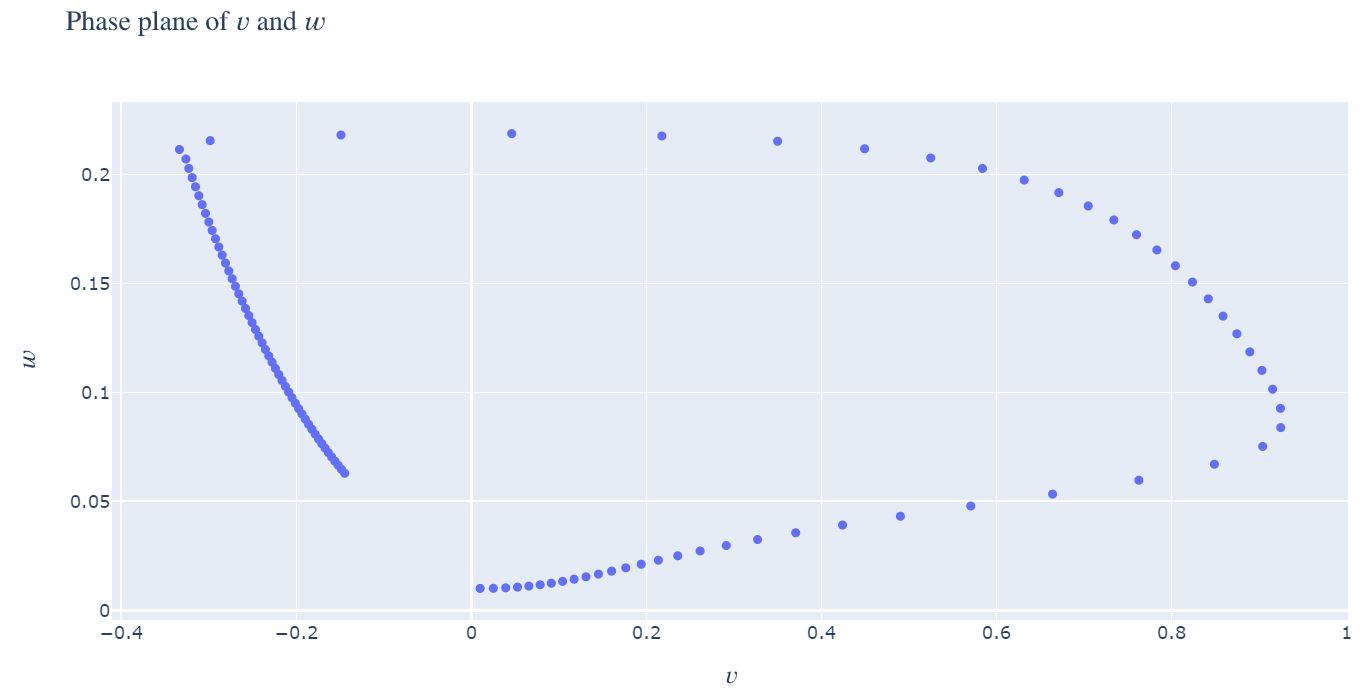
\includegraphics[width=0.95\columnwidth]{FHN_Euler_explicit_phase_plane}
    \caption{Phase plane of $v$ and $w$ by Euler's explicit method.}
    \label{fig:Euler_explicit_phase_plane}
\end{figure}

\begin{figure}
    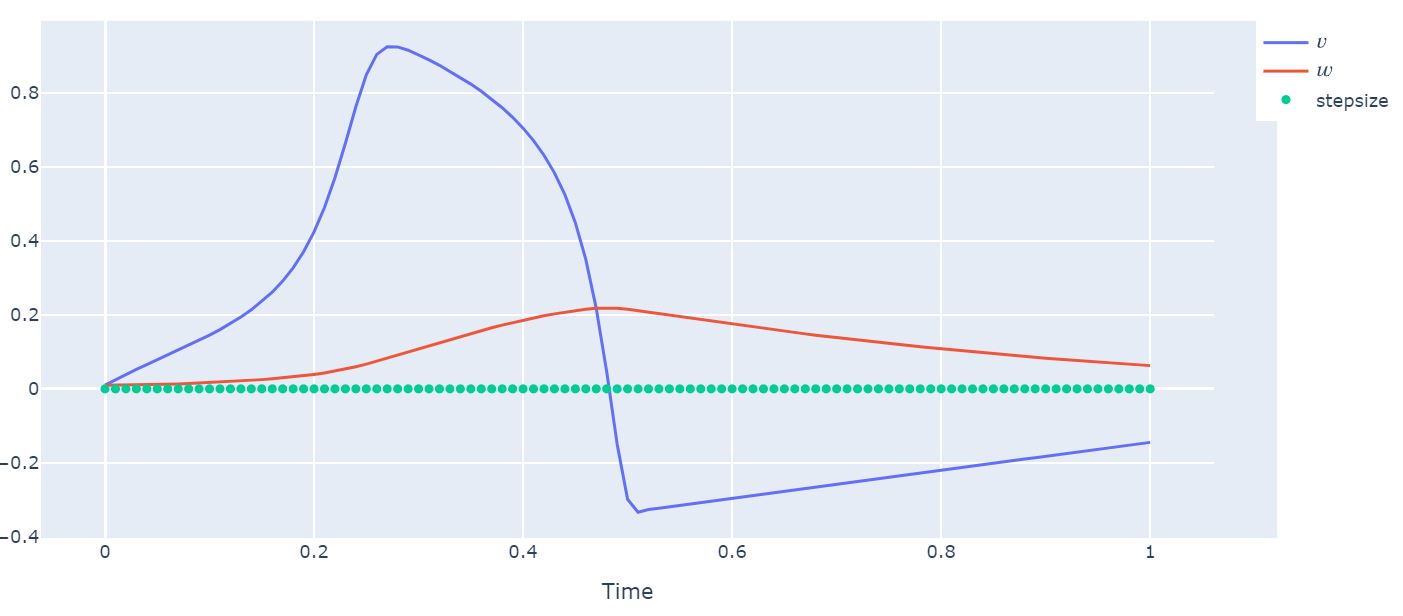
\includegraphics[width=0.95\columnwidth]{FHN_Euler_explicit_variable}
    \caption{Graph of $v$ and $w$ against time by Euler's explicit method.}
    \label{fig:Euler_explicit_variable}
\end{figure}


From Figure \ref{fig:Euler_explicit_variable}, we can see that $v$, the excitation variable is excited in the early stage. While $v$ increases significantly, the change in $w$ is small. After $v$ reaches its peak and starts to reduce, $w$ increases slowly. This can be observed in both the phase plane (Fig. \ref{fig:Euler_explicit_phase_plane}) and the variable graph (Fig. \ref{fig:Euler_explicit_variable}). When the variable $v$ starts to recover to its original value, $w$ is at its maximum. The scattering of points in the phase plane captures the feature of the model, where the change in $v$ is rapid while the change in $w$ is slow. When the change in $v$ is significantly larger than the change in $w$, the points are sparse. On the other hand, the points are packed when $w$ increases or decreases more than $v$. However, in the adaptive methods, such insights cannot be interpreted directly from the phase plane. Therefore, green triangles were plotted in Fig. \ref{fig:adaptive_variable} to indicate the adapted mesh points. The mesh points are adapted towards large difference in $v$ or $w$ over a short period of time.

\begin{figure}
    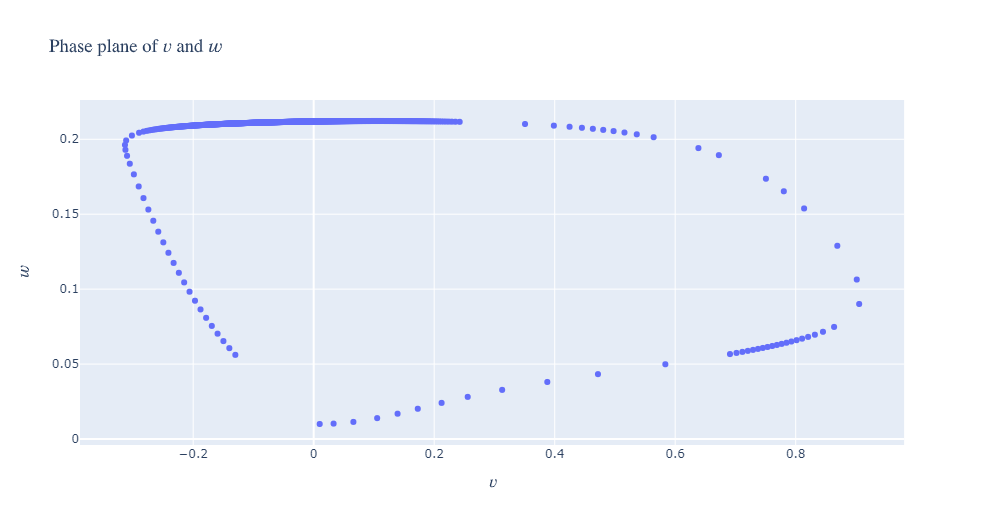
\includegraphics[width=0.95\columnwidth]{FHN_adaptive_phase_plane}
    \caption{Phase plane of $v$ and $w$ for adaptive method BS23.}
    \label{fig:adaptive_phase_plane}
\end{figure}

\begin{figure}
    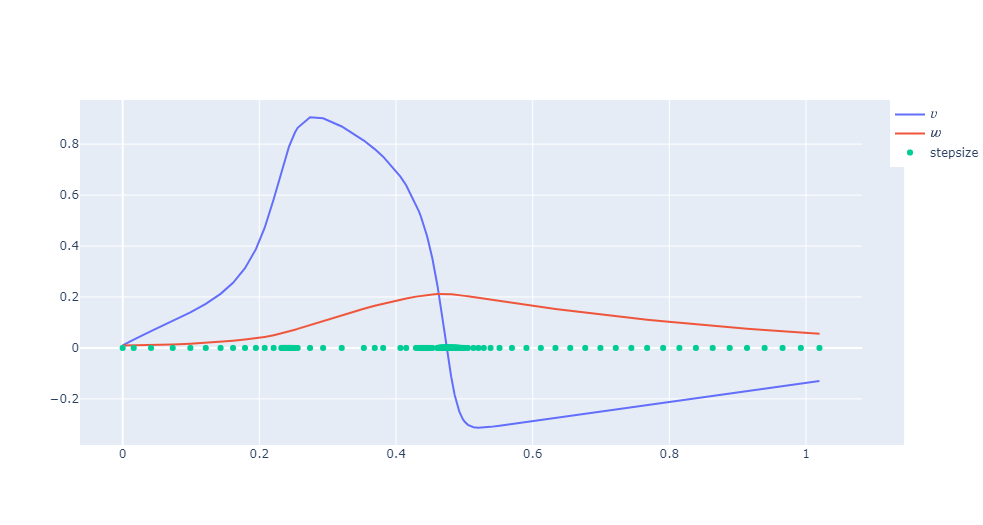
\includegraphics[width=0.95\columnwidth]{FHN_adaptive_variable}
    \caption{Graph of $v$ and $w$ against time for adaptive method BS23}
    \label{fig:adaptive_variable}
\end{figure}

\section{Convergence of Fitzhugh-Nagumo model}
\label{sec:FHN-convergence}
A notebook (access from the link: \href{https://nbviewer.jupyter.org/github/FarmHJ/numerical-solver/blob/main/examples/fhn_model_convergence.ipynb}{\underline{\emph{Fitzhugh-Nagumo convergence notebook}}} is created to test the convergence of the solution to the Fitzhugh-Nagumo model. Since the model has no analytical solution, it is tested against a reference solution. The reference solutions are assumed to be sufficiently accurate. For methods with fixed step size, which are the one-step methods and predictor-corrector method, the reference solutions are constructed by using a smaller step size. For methods with adaptive step size, reference solutions are obtained by using a smaller tolerance value. This notebook shows the numerical solution computed for different methods at different step sizes or tolerance values. The numerical solutions are then compared with their respective reference solutions. In both methods, the error decreases as step size or tolerance decreases.

\begin{figure}
    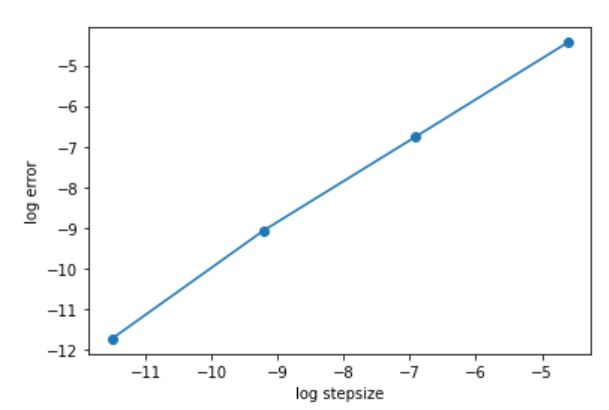
\includegraphics[width=0.95\columnwidth]{FHN_Euler_explicit_error_behaviour}
    \caption{Error at a mesh point for Euler's explicit method.}
    \label{fig:Euler_explicit_error}
 \end{figure}
\begin{figure}
   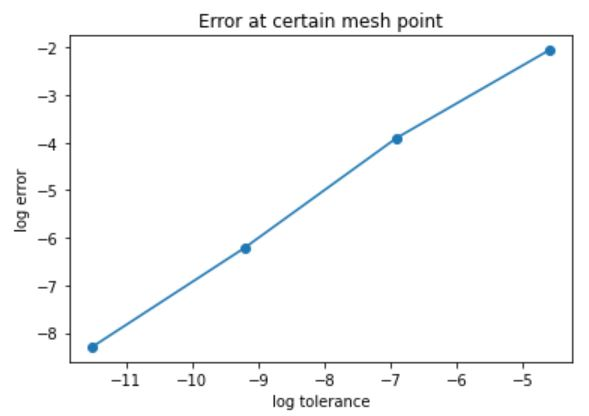
\includegraphics[width=0.95\columnwidth]{FHN_adaptive_error_behaviour}
   \caption{Sum of error for adaptive method BS23.}
   \label{fig:adaptive_error}
\end{figure}